% gemma-csm paper. Self-contained: compiles with a standard TeX install.
% Build:  tectonic main.tex   (or: latexmk -pdf main.tex)
\documentclass[11pt]{article}

\usepackage[utf8]{inputenc}
\usepackage[T1]{fontenc}
\usepackage{microtype}
\usepackage[margin=1in]{geometry}
\usepackage{amsmath,amssymb}
\usepackage{graphicx}
\usepackage{booktabs}
\usepackage{float}
\usepackage{url}
\usepackage[hidelinks]{hyperref}
\usepackage[numbers,sort&compress]{natbib}
\usepackage{xcolor}

% give floats (tables/figures) room to breathe from body text
\setlength{\textfloatsep}{16pt plus 3pt minus 3pt}
\setlength{\intextsep}{16pt plus 3pt minus 3pt}
% let TeX break long \texttt{} identifiers instead of running into the margin
\emergencystretch=3em

\title{Conversational Speech Generation on an Encoder-Free\\ Multimodal Backbone}
\author{Gianni Sanrochman\\ \texttt{gsanrochman@proton.me}}
\date{\today}

\begin{document}
\maketitle

\begin{abstract}
Speech-capable language models usually bolt a separate audio encoder onto a text
LLM. We ask a narrower question: is a frozen multimodal LLM's \emph{own},
encoder-free audio pathway enough, and can lightweight adapters alone give it a
voice? We couple a frozen Gemma-4 backbone with a CSM-style speech head, a
semantic-codebook predictor plus a depth transformer over Mimi
residual-vector-quantized codes, and train only QLoRA adapters and the head on a
single 16\,GB GPU. \textbf{(RQ1)} On the smaller E2B backbone the recipe teaches a
fully frozen, quantized LLM to speak: \textbf{13\% word error rate, 88\% word
recall} on held-out text-to-speech. \textbf{(RQ2)} For the encoder-free 12B
backbone we characterize \emph{how} audio must reach it. (i)~Naive 4-bit NF4
quantization \emph{silently destroys the backbone's audio comprehension} (held-out
transcription word recall falls from \textbf{0.65 to 0.12}) while sparing prosody;
keeping only the audio tower and projector in bf16 (a ${\sim}10.5$\,GB hybrid load)
restores it. (ii)~\emph{Delivery matters}: the native multimodal pathway conveys
lexical content, whereas a hand-built feature-splice of the same features conveys
prosody but not content. Exploiting these, a two-stage cascade (native
understanding into the frozen backbone, then the speech head) gives
\emph{conversational speech-to-speech with no backbone training}, rendering
held-out replies at \textbf{13.1\% WER / 91.9\% recall}. (iii)~But
prosody-conditioning, replying based on \emph{how} the query was said, is not yet
realized: output prosody shows only a weak loudness echo, with no pitch or timing
tracking. Two methodological findings recur: teacher-forced codebook cross-entropy
is \emph{not} a proxy for free-running intelligibility (a memorizing model scores
well yet decodes at 141\% WER), so word error rate on decoded audio is the
necessary gate; and the Mimi codec imposes an entropy floor that cross-entropy
cannot cross. We further collapse the cascade into a \emph{single} end-to-end model
that delivers audio natively and conditions the speech head on the backbone's latent
reply: it speaks intelligible, grounded, full-length replies in one forward pass
(WER~0.00 on the best held-out clips). A controlled ablation, however, shows heavy
adapter training on limited data erodes the backbone's out-of-distribution
competence: the frozen backbone's intelligence stays intact (disabling the adapter
restores it), but the adapter masks it, making robustness a data-and-adaptation
problem rather than an architectural one. Code, checkpoints, and data are released.
\end{abstract}

\section{Introduction}
\label{sec:intro}
Multimodal language models are usually extended to speech by attaching a separate
audio encoder, typically a Whisper variant, to the language model and projecting
its features into the token stream. That recipe is effective but heavy: it adds an
encoder, treats audio as a foreign modality to be translated in, and is rarely
trainable on a single consumer GPU. Recent backbones such as Gemma-4 are instead
\emph{encoder-free}: they ingest audio through the model's own multimodal pathway
with no external encoder, which sharpens the question. If the backbone already
\emph{understands} audio natively, is that pathway enough to also give it a
\emph{voice} using only lightweight adapters: no encoder, no backbone fine-tuning,
on 16\,GB? We keep the language model frozen, keep its native audio pathway, and
learn only a small speech-output head plus low-rank adapters.

\paragraph{Research questions.}
\begin{itemize}
  \item \textbf{RQ1 (foundation).} Can lightweight adapters teach a frozen 4-bit
        LLM to generate intelligible speech at all? We answer yes on the E2B
        backbone (\S\ref{sec:rq2}).
  \item \textbf{RQ2 (thesis).} Using the backbone's \emph{encoder-free} audio
        input, can the model produce a spoken response conditioned on \emph{how}
        the query was said (prosody, emotion), not merely what was said?
\end{itemize}
A negative RQ1 would not damage RQ2; a positive RQ1 is independently useful, a
cheap way to give an already-deployed frozen LLM a voice.

\paragraph{Contributions.}
\begin{enumerate}
  \item An encoder-free recipe coupling Gemma-4's native audio features with a
        CSM-style speech head (semantic codebook plus a depth transformer over
        Mimi RVQ codes), trainable end-to-end under QLoRA on 16\,GB.
  \item Evidence for RQ1: a fully frozen, quantized LLM made to speak
        intelligibly (13\% WER / 88\% recall) by adapters alone (\S\ref{sec:rq2}).
  \item A quantization finding: 4-bit NF4 quantization of the \emph{whole}
        backbone silently destroys its audio comprehension while sparing prosody;
        protecting only the audio tower and projector in bf16 restores verbatim
        understanding at ${\sim}10.5$\,GB (\S\ref{sec:quant}).
  \item A delivery finding: the backbone's native multimodal audio pathway
        conveys lexical content, whereas a hand-built feature-splice of the same
        features conveys prosody but not content, isolating audio \emph{delivery},
        not quantization or capacity, as the bottleneck (\S\ref{sec:delivery}).
  \item A working demonstration of RQ2: a two-stage cascade (native understanding
        $\to$ frozen-backbone CSM speech head) holds a relevant spoken
        conversation with \emph{no backbone training}, rendering held-out replies
        at \textbf{13.1\% WER / 91.9\% recall}; a head-refinement run fixes
        word-onset dropping (\S\ref{sec:cascade}). Prosody conditioning, replying
        to \emph{how} the query was said, is \emph{not} yet realized: output
        prosody shows only a weak loudness echo, a clean negative bound
        (\S\ref{sec:prosody}).
  \item A \emph{single} end-to-end model collapsing the cascade: native audio
        delivery with the speech head conditioned on the backbone's own latent
        reply, speaking intelligible, grounded, full-length replies in one forward
        (WER~0.00 on the best held-out clips). A three-way ablation localizes its one
        weakness, out-of-distribution template collapse, to adapter overfitting,
        not the architecture: the frozen backbone's intelligence stays intact and is
        restored by disabling the adapter. A hybrid that ablates only the
        content-selection pass then voices the reply with the adapter on recovers
        correct content with largely intelligible speech, with no retraining
        (\S\ref{sec:unified}).
  \item A methodological finding: teacher-forced codebook cross-entropy ($c_0$)
        is not a proxy for free-running intelligibility (and the same trap recurs
        for comprehension); word error rate on decoded audio is the necessary gate
        (\S\ref{sec:findings}).
  \item A characterization of the Mimi codec entropy floor that caps naturalness
        under cross-entropy training (\S\ref{sec:codecfloor}).
\end{enumerate}

\section{Related Work}
\label{sec:related}
\paragraph{Speech and audio LLMs.}
Most speech-capable LLMs attach a separate audio encoder to a text LM. On the
understanding side, SALMONN~\citep{tang2024salmonn} fuses Whisper~\citep{radford2023whisper}
and BEATs encoders into a frozen LLM via a Q-Former, and Qwen-Audio~\citep{chu2023qwenaudio}
couples a Whisper-style encoder to an LLM; both are speech-in, text-out. For
speech \emph{generation}, a dominant line discretizes audio into units or codec
tokens: GSLM~\citep{lakhotia2021gslm} models raw-audio units, VALL-E~\citep{wang2023valle}
is a codec-token LM for text-to-speech, and SpeechGPT~\citep{zhang2023speechgpt}
and AudioPaLM~\citep{rubenstein2023audiopalm} extend an LLM's vocabulary with
speech units and fully (re)train. Full-duplex models such as
Moshi~\citep{defossez2024moshi} train a bespoke speech backbone with the Mimi
codec, while LLaMA-Omni~\citep{fang2024llamaomni} adds a speech adaptor and
streaming decoder atop an LLM but still bolts a Whisper encoder on the input. We
differ on four axes: (i)~no external audio encoder, we use Gemma-4's
\emph{native} audio pathway; (ii)~the backbone stays frozen, adapted only by
QLoRA plus a speech head on a single 16\,GB GPU; (iii)~bidirectional
conversational speech; and (iv)~we gate on free-running WER rather than
teacher-forced loss (\S\ref{sec:findings}).

\paragraph{Frozen-backbone and text-free speech-to-speech.}
Three recent systems bracket our setting. Freeze-Omni~\citep{wang2024freezeomni}
also keeps the LLM frozen, but, like our cascade, routes a streaming speech
\emph{encoder} into the LM on input and drives an autoregressive speech decoder
from the LM's \emph{textual} response on output: a frozen-LLM, text-mediated
pipeline whose stated motivation, avoiding catastrophic forgetting under limited
data, is exactly ours. Qwen2.5-Omni~\citep{xu2025qwen25omni} removes that text
bottleneck with its Thinker--Talker design, the Talker ``directly utilizes the
hidden representations from the Thinker to produce audio tokens'', but trains
\emph{end-to-end} rather than freezing the backbone. Concurrent with our work,
MOSS-Speech~\citep{zhao2025mossspeech} reaches true text-free speech-to-speech on
an initially frozen backbone by carving modality-specific layers into the
transformer itself: of Qwen3-8B's 36 layers the first 32 form a shared trunk and
the last four split into parallel text- and speech-prediction stacks, trained with
the backbone frozen before a later partial unfreeze. Relative to all three, our
study occupies a distinct point: native \emph{continuous}-audio input (no discrete
speech tokenizer and no external encoder), a backbone that stays \emph{fully}
frozen, and training confined to QLoRA plus a small external head on a single
16\,GB GPU. We obtain the conversational loop through the same frozen-LLM,
text-mediated cascade as Freeze-Omni, and report an honest negative result on the
naive single-model bolt-on (\S\ref{sec:cascade}); the hidden-state conditioning of
Qwen2.5-Omni and the in-trunk modality split of MOSS-Speech both indicate why it
failed and chart the route for collapsing our cascade into one network
(\S\ref{sec:discussion}).

\paragraph{Parameter-efficient adaptation of frozen models.}
We freeze the backbone and train only adapters: LoRA~\citep{hu2022lora} (here in
its 4-bit QLoRA form~\citep{dettmers2023qlora}) and bottleneck
adapters~\citep{houlsby2019adapters}. This follows the ``freeze the LLM, add a
small bridge'' paradigm of Flamingo~\citep{alayrac2022flamingo} and
LLaVA~\citep{liu2023llava}, but for audio in \emph{and} out and \emph{without} a
separate modality encoder.

\paragraph{Conditioning frozen LMs on new modalities.}
Closest to our setting, \citet{penov2026loraBridges} adapt a frozen small
language model to sensor streams (vision, audio, IMU) via conditional LoRA
bridges: a hypernetwork generates LoRA weights at runtime from a frozen sensor
encoder's features. We share the premise of adapting a frozen quantized LLM to a
non-text input without retraining the backbone, but differ in mechanism and goal:
(i)~we use the backbone's native, encoder-free audio pathway rather than a
separate sensor encoder feeding a weight-generating hypernetwork; (ii)~our
adapters are fixed LoRA plus dedicated speech-output heads, not input-conditioned
generated weights; and (iii)~we target bidirectional conversational speech (audio
in and out). Methodologically their study and ours converge on the same warning
(\S\ref{sec:findings}): an aggregate language-modeling loss does not measure the
capability of interest, and a task-grounded probe is required.

\section{Method}
\label{sec:method}

\begin{figure}[t]
\centering
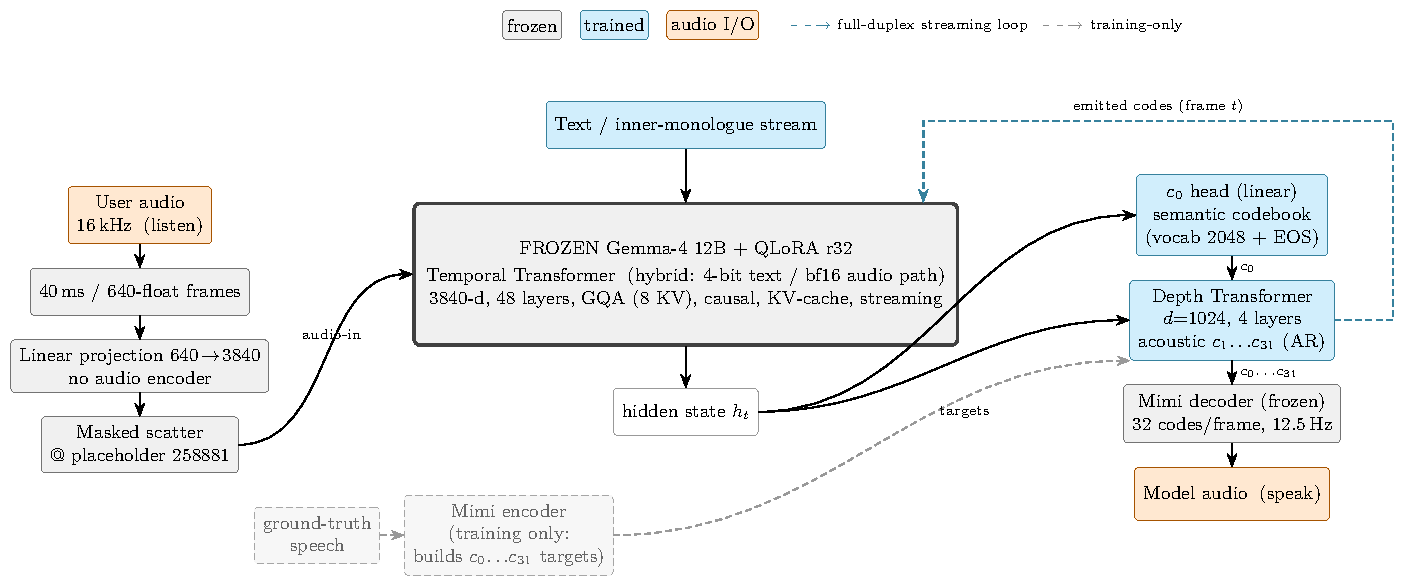
\includegraphics[width=\linewidth]{figures/architecture.pdf}
\caption{Architecture of the full-duplex conversational model. The frozen
Gemma-4 12B decoder (the \emph{Temporal Transformer}) is the only large
component; the trainable parameters are the QLoRA adapters, the audio-frame
embedding tables, the $c_0$ head, and the depth transformer. The understanding
(listen) path is \emph{encoder-free}: incoming audio is sliced into
40\,ms / 640-float frames, linearly projected $640\!\to\!3840$, and scattered
into the decoder at audio placeholder tokens, with no ASR/audio encoder. The
generation (speak) path emits Mimi codes, a linear $c_0$ head for the semantic
codebook and a depth transformer for the 31 acoustic codebooks, which the frozen
Mimi decoder renders to waveform; \emph{at inference no encoder runs on audio.}
The Mimi encoder is used only at training time, to build the $c_0\!\dots\!c_{31}$
targets. The dashed loop is the full-duplex streaming path: the model's emitted
codes at frame $t$ are embedded as audio-out input at frame $t{+}1$, so listening
and speaking proceed frame-synchronously. This is the \emph{target}
single-model layout; we demonstrate both the two-stage cascade of
\S\ref{sec:cascade} (native-pathway understanding $\to$ this speak head) and the
unified end-to-end model of \S\ref{sec:unified}, audio delivered through the native
pathway inside one network, the head conditioned on the backbone's latent reply. The
understanding path
requires the audio tower and projector in bf16 (\S\ref{sec:quant}); only the
language layers are 4-bit. Full duplex is the streaming extension of the
\texttt{[text $\mid$ audio-in $\mid$ audio-out]} layout.}
\label{fig:arch}
\end{figure}

\subsection{Encoder-free backbone}
Figure~\ref{fig:arch} shows the full architecture.
We build on Gemma-4 12B ``Unified''~\citep{gemma4_2026}, Google's encoder-free
multimodal variant: 16\,kHz audio is sliced into 40\,ms / 640-float frames and
linearly projected into the decoder's hidden space ($640\to3840$, one-to-one in
time), merged at audio placeholder tokens (token id $258881$) via a masked
scatter into the input embeddings. There is no separate ASR/audio encoder; we
access these projected features through the model's \texttt{get\_audio\_features}.
The smaller E2B/E4B audio variants instead use a USM conformer encoder and are
\emph{not} encoder-free; our encoder-free claim is specific to the 12B. The 12B
decoder is 3840-dimensional, 48 layers, grouped-query attention (8 KV heads), with
no per-layer-embedding tables and no KV-sharing.

\subsection{Speech-output head}
Audio is represented as Mimi codes~\citep{defossez2024moshi}: a streaming
split-RVQ codec at 12.5\,Hz whose released checkpoint provides 32 codebooks
(1 semantic, 31 acoustic). Following the CSM head topology~\citep{sesame2025csm},
a linear semantic head predicts codebook 0 ($c_0$, vocabulary $2048$ plus an
end-of-speech token) and a depth transformer (a causal transformer, $d{=}1024$,
4 layers, 8 heads) autoregressively predicts the remaining 31 acoustic codebooks
conditioned on the pre-frame hidden state and the sampled $c_0$. The loss is
$\mathcal{L}_{c_0} + \lambda\,\mathcal{L}_{\text{depth}}$ with the depth term
computed on a random subset of frames per step (we use $1/16$ to $1/4$). Each
audio frame's input embedding is the sum of its 32 codebook embeddings (new
tables, untied, unlike CSM). Unlike CSM (a from-scratch Llama backbone) we attach
this head to the frozen Gemma-4 decoder. The sequence layout is
\texttt{[text $\mid$ audio-in $\mid$ audio-out frames]}; the hidden state at the
last text position predicts the first output frame, and frame $t$ predicts frame
$t{+}1$ (shifted next-frame prediction).

\subsection{QLoRA training on 16\,GB}
The backbone is frozen in 4-bit NF4 with double quantization and bf16 compute;
the Mimi codec is frozen. The trainable parameters are the LoRA
adapters~\citep{dettmers2023qlora} (rank 32, applied to all linear layers,
attention and MLP, following a coverage-over-rank principle), the audio-frame
embedding tables, the $c_0$ head, and the depth transformer. We optimize with
PagedAdamW8bit, batch size 1 with gradient accumulation 16, gradient
checkpointing, and a per-clip frame cap. We sample at evaluation with temperature
0.6--0.9 and top-$k$ 50 (cooler settings yield longer intelligible output).

\subsection{Curriculum: Phase A then Phase B}
Phase A (text$\to$speech) teaches the head to speak on clean read speech; Phase B
turns the audio input on and learns understanding-conditioned response on
conversational query/response audio. The order is forced: Phase B resumes from a
model that can already speak, so audio-conditioning has speech to attach to. A key
lesson (\S\ref{sec:findings}) is that Phase A needs the \emph{volume} of a large
clean corpus (LibriTTS), not a small conversational set; the latter merely
memorizes.

\section{Experimental Setup}
\label{sec:setup}
\paragraph{Hardware.} All training runs on a single 16\,GB consumer GPU
(${\sim}15.4$\,GB usable). The frozen 12B loads at ${\sim}10.6$\,GB; capped-sequence
audio-in training fits at ${\sim}13.7$\,GB. The decisive memory levers are batch-1
with gradient accumulation, SDPA attention (eager materializes $O(\text{seq}^2)$
fp32 attention), a headless display, and \texttt{max\_split\_size\_mb:256}; note
that \texttt{expandable\_segments} is incompatible with bitsandbytes 4-bit kernels
and silently no-ops. A single ${\sim}\$7$ rented-A100 session was used for one
larger E2B run; that workload is memory-bound, so the A100 gave only ${\sim}1.5\times$
the consumer-card throughput, not the nominal compute ratio.

\paragraph{Data.} Phase A trains on a ${\sim}110$\,h / 90.6k-clip subset of
LibriTTS~\citep{zen2019libritts} (24\,kHz, CC BY 4.0). Phase B uses the English
split of OpenS2S~\citep{casia2025opens2s} (Apache-2.0): 49{,}368 paired
(audio-query, audio-response) examples with transcripts and emotion labels. We
re-encode all response audio with Mimi at 12.5\,Hz (OpenS2S itself ships raw WAVs
tokenized with GLM-4-Voice, which we do not use).

\paragraph{Evaluation.} We decode free-running (the model consumes its own
sampled frames), transcribe with faster-whisper, normalize both reference and
hypothesis with the standard English text normalizer, and report WER and
\emph{word recall} (the fraction of reference words present in the hypothesis,
a multiset measure that is immune to the insertions that drive WER above 100\% at
low intelligibility). Double-blind human listening is the gold reference; it
agrees closely with the recall harness.

\section{Results}
\label{sec:results}
\subsection{RQ1: adapters teach a frozen LLM to speak}
\label{sec:rq2}
We establish RQ1 on the smaller E2B backbone (text$\to$speech; with no audio
input involved, the encoder-free distinction does not apply here).

\textbf{Intelligibility (M3).} Trained on ${\sim}840$\,h (LibriTTS-R plus
LJSpeech), the frozen 4-bit LLM with QLoRA adapters and the speech head reached a
final-checkpoint mean battery word-recall of \textbf{71\%}, with multiple novel
sentences at 100\% recall (e.g.\ ``Please close the door before you leave'');
train/val $c_0$ were 2.54/2.65 with no overfitting gap. To our knowledge this is
the first demonstration of intelligible speech from a fully frozen, quantized LLM
via parameter-efficient adaptation alone, produced on a single 16\,GB GPU plus a
${\sim}\$7$ rented-A100 session.

\textbf{Duration (M4).} A same-speaker concatenation phase (mean ${\sim}18$\,s
clips) cured early truncation: speech sustains ${\sim}11$--$13$\,s at 86--90\%
voiced. The final 10-clip battery scored \textbf{mean WER 13\%, word-recall 88\%}
(novel sentences 91\%/9\%; reused probes 84\%/17\%), with $c_0\approx2.15$.
Residual errors are acoustic, not lexical (``lazy goat''/dog).

\textbf{Human--machine agreement.} Double-blind human transcription tracked the
recall harness closely (human 14--22\% vs.\ machine ${\sim}18$\% in the M2 era),
supporting free-running WER/recall as the quality gate rather than teacher-forced
loss.

\subsection{RQ2: from naive integration to a working cascade}
\label{sec:rq1}
The 12B encoder-free pipeline is validated end-to-end: a training step consumes
\texttt{[text $\mid$ audio-in $\mid$ audio-out]} with audio features from
\texttt{get\_audio\_features} and propagates gradients at a 13.7\,GB peak, and a
text-conditioned speech head trained this way voices supplied replies near
verbatim. But making the frozen backbone respond to \emph{what the query said}
(content), not only \emph{how} (prosody), exposed two failure modes that we had to
isolate before a conversational system worked.

\subsubsection{4-bit quantization destroys audio comprehension}
\label{sec:quant}
The RQ1 recipe loads the entire backbone in 4-bit NF4. Probing the 12B's audio
understanding through its \emph{native} multimodal chat-template, the 4-bit model
transcribes nothing and answers generically (e.g.\ ``You haven't said anything
yet'') regardless of the spoken input; the same probe in full bf16 transcribes
verbatim (``The quick brown fox\ldots''; a spoken name and a spoken question
correctly answered). The cause is that bitsandbytes quantizes the audio tower and
audio projector along with the language layers, while the library's automatic
skip list protects only tied/output embeddings. Listing the audio tower,
\texttt{embed\_audio}, the vision modules, and \texttt{lm\_head}/\texttt{embed\_tokens}
in \texttt{llm\_int8\_skip\_modules} keeps the audio pathway in bf16 (a ${\sim}10.5$\,GB
``hybrid'' load that still fits 16\,GB) and restores verbatim understanding.
Notably, \emph{prosody} conditioning survived 4-bit (RQ2's original framing
worked), but lexical content did not, so every earlier ``comprehension'' failure
was this single artifact. Table~\ref{tab:quant} quantifies it: on 40 held-out
OpenS2S queries, asking the model to transcribe the audio recovers 65\% of content
words in bf16 but only 12\% in naive 4-bit, where the model typically refuses
(``I cannot provide a transcription because there is nothing\ldots''). We report
word recall (content overlap) as the robust metric because the bf16 model
paraphrases rather than transcribes verbatim, inflating its WER; the recall gap
isolates the quantization effect.

\begin{table}[tbp]\centering
\caption{Does the frozen backbone receive the spoken \emph{content}? Free-running
transcription of 40 held-out OpenS2S queries (normalized), through the native
multimodal pathway, at bf16 vs.\ naive whole-model 4-bit NF4. Word recall is the
fraction of reference words present in the output.}
\label{tab:quant}
\begin{tabular}{llcc}\toprule
delivery & precision & word recall & WER \\ \midrule
native pathway & bf16 & \textbf{0.65} & 0.62 \\
native pathway & 4-bit NF4 (naive) & \textbf{0.12} & 1.34 \\ \bottomrule
\end{tabular}
\end{table}

\subsubsection{Delivery mechanism: native pathway vs.\ feature-splice}
\label{sec:delivery}
Even with the audio path in bf16, \emph{how} features enter the decoder decides
whether content survives. We compare two deliveries of the identical audio
features: (a)~our hand-built path, which calls \texttt{get\_audio\_features} and
splices the projected frames into \texttt{[BOS $\mid$ audio $\mid$ text]} (used since
Phase B, and which carries prosody); and (b)~the processor's native chat-template,
which inserts audio soft-tokens and merges them by masked scatter. The splice path
produces hallucinated transcripts, the model invents a fluent, unrelated query
and answers \emph{that} (free-running transcript WER ${\sim}1.1$), whereas the
native path transcribes verbatim. Having eliminated training instability
(\S\ref{sec:stability}), quantization (\S\ref{sec:quant}), and capability (the
native path understands), we isolate audio \emph{delivery} as the bottleneck: the
manual splice transmits prosody but not lexical content.

\subsubsection{End-to-end ``inner monologue'' attempts fail informatively}
\label{sec:monologue}
We first tried a single model that both understands and speaks. A \emph{joint}
layout \texttt{[audio $\mid$ reply-text $\mid$ reply-audio]} with loss on text and
audio produced on-style but generic, off-topic replies: because the reply text is
always present in the prefix (no text dropout), the objective rewards
\emph{vocalizing a supplied answer}, never \emph{deciding} what to say, visible
only under a text-free decode, not in the loss. A \emph{grounded} variant adding a
comprehension loss (transcribe the query, whose transcript already ships in the
data) drove teacher-forced comprehension loss to ${\sim}0.5$ while free-running
transcript WER stayed at $1.07$--$1.13$: the model hallucinates a fluent unrelated
query and replies to it, the $c_0$-is-not-intelligibility trap
(\S\ref{sec:findings}), now recurring for \emph{comprehension}. These negatives
motivate decoupling understanding (native pathway) from speaking (the validated
head).

\subsubsection{A working cascade, and head refinement}
\label{sec:cascade}

\begin{figure}[t]
\centering
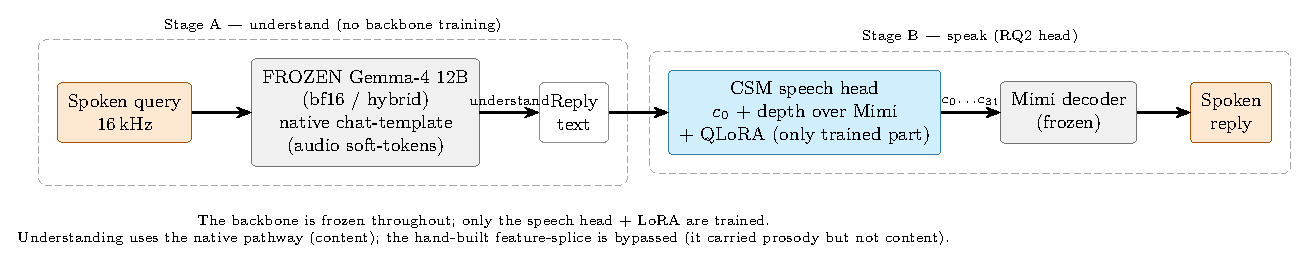
\includegraphics[width=\linewidth]{figures/cascade.pdf}
\caption{The two-stage conversational cascade (\S\ref{sec:cascade}). Stage~A feeds
the spoken query to the frozen backbone through its \emph{native} multimodal
pathway and reads out a reply in text; Stage~B is the CSM-style speech head (the
RQ1 text$\to$speech head) that voices the reply, rendered to waveform by the frozen
Mimi decoder. The backbone is frozen throughout and the hand-built feature-splice
(\S\ref{sec:delivery}) is bypassed for understanding; only the speech head and LoRA
are trained. Collapsing this into one network via native delivery is the remaining
step.}
\label{fig:cascade}
\end{figure}

Combining the two diagnoses gives a system that needs \emph{no backbone training}
(Figure~\ref{fig:cascade}).
Both stages are the \emph{same} frozen backbone, one set of weights, invoked
twice, so the cascade is already a single model in \emph{parameters}; ``two-stage''
names the information path, two forward passes joined by a discrete-text handoff.
The ``single end-to-end model'' we target therefore removes not a second network
but that text bottleneck: one forward pass in which the speech head conditions on
the hidden states the backbone produces while natively ingesting the query, so
prosody and paralinguistics can survive into the reply rather than being discarded
at the text interface.
Stage~A is the frozen backbone in bf16/hybrid, fed audio through the native
chat-template, emitting a reply \emph{text}. Stage~B is the CSM-style speech head
(the RQ1 text$\to$speech head) voicing that reply. On a small conversational
battery the cascade closes the loop on-topic and intelligibly (a promotion query
$\to$ a congratulation; ``I've been feeling overwhelmed'' $\to$ an empathetic
reply), bypassing the broken splice for understanding while reusing the proven head
for voice. A short head-refinement run (8k steps, warm-started, on the hybrid
backbone) then removed a residual artifact in which the head dropped the first one
to three words: clean verbatim rendering rose from 1/3 to 3/3 of the battery, and
output extended to clean ${\sim}13$--$20$\,s multi-sentence replies; an
out-of-distribution probe (a spoken self-introduction absent from training) was
understood and voiced verbatim, with only an occasional sentence-initial word
substitution remaining on rare words. Across this run teacher-forced validation
loss was flat while free-running quality jumped from 1/3 to 3/3, the $c_0$ trap
once more. Table~\ref{tab:cascade} summarizes the battery. At scale, on 40
held-out OpenS2S queries, the cascade renders the Stage-A reply at \textbf{13.1\%
WER and 91.9\% word recall} (free-running, faster-whisper-normalized), matching the
RQ1 text-to-speech intelligibility (\S\ref{sec:rq2}).

\begin{table}[tbp]\centering
\caption{Cascade conversational battery: free-running output transcribed with
faster-whisper and compared to the Stage-A reply text. Understanding (Stage~A,
full-bf16 native pathway) is held fixed; only the Stage-B head varies.
\emph{Onset}~$=$ leading word(s) rendered; \emph{verbatim}~$=$ full reply with no
word error. This per-clip battery illustrates the failure modes; the aggregate
held-out result (40 queries: 13.1\% WER, 91.9\% recall) is reported in the text.}
\label{tab:cascade}
\small
\begin{tabular}{llccp{3.4cm}}\toprule
Battery & Stage-B head & onset & verbatim & residual \\ \midrule
short (3, ${\sim}3$\,s)       & pre-refinement & 1/3 & 0/3 & dropped 1--3 leading words; one stutter \\
short (3, ${\sim}3$\,s)       & refined        & 3/3 & 3/3 &, \\
long (3, 13--20\,s)           & refined        & 2/3 & 2/3 & one sentence-initial substitution \\
OOD (unseen self-intro)       & refined        & 1/1 & 1/1 & rare-word subs.\ when long \\ \bottomrule
\end{tabular}
\end{table}

\subsection{Collapsing the cascade: a demonstrated unified model and its limit}
\label{sec:unified}
We then built the single end-to-end model the cascade points to. \texttt{forward\_unified}
delivers the query audio through the backbone's \emph{native} multimodal forward
(\texttt{<audio>} placeholders $+$ \texttt{input\_features}, the path proven to carry
lexical content in \S\ref{sec:delivery}) and conditions the CSM head on the hidden
states of the autoregressively generated reply, one forward pass, no text
re-encoding, in the spirit of Qwen2.5-Omni's Thinker--Talker~\citep{xu2025qwen25omni}.
Only LoRA and the head are trained (backbone frozen); the head is warm-started from
the cascade's and the model is trained on the full English OpenS2S split
(4{,}898 pairs, 3{,}000 steps, on a rented A6000 because the gradient-checkpointing-off
native forward exceeds 16\,GB at full reply length).

\begin{figure}[tbp]
\centering
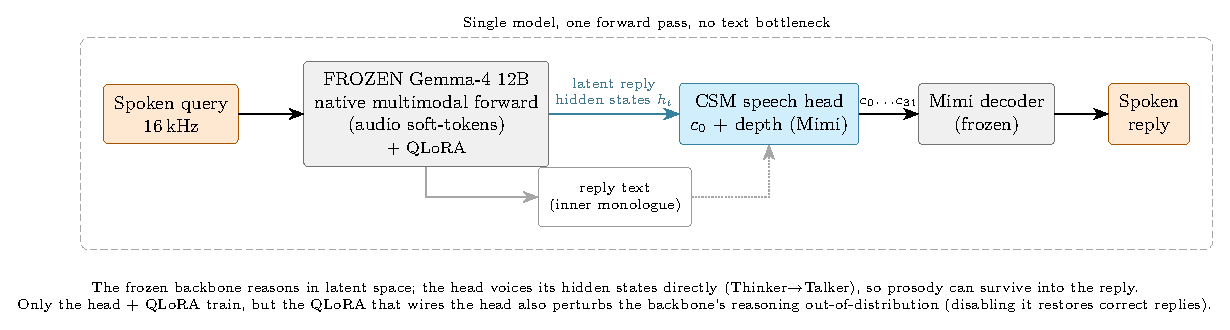
\includegraphics[width=\linewidth]{figures/unified.pdf}
\caption{The unified single model (\S\ref{sec:unified}). The frozen encoder-free
backbone ingests the spoken query through its \emph{native} multimodal forward and
the CSM speech head is conditioned on the \emph{hidden states} of the
autoregressively generated reply, the model's own latent reasoning, rather than on
re-encoded text, so understanding and speaking happen in one forward pass with no
text bottleneck (Qwen-style Thinker$\to$Talker). Only the head and QLoRA are trained;
the backbone is frozen. The honest caveat (\S\ref{sec:unified}): the QLoRA that wires
the head onto the latent also perturbs the backbone's reasoning out-of-distribution,
which a three-way ablation localizes (disabling the adapter restores correct replies).}
\label{fig:unified}
\end{figure}

\paragraph{It works: single-pass, intelligible, grounded.} On held-out OpenS2S
queries the unified model produces \emph{full-length} (9--12\,s) spoken replies that
free-running faster-whisper recovers near-verbatim (\textbf{WER 0.00} on the best
clips, $0.03$--$0.29$ typical) in a single forward, with no text bottleneck. A
zeroed-audio ablation, replacing the input features with zeros, changes the reply
every time, confirming the output is grounded in the audio and not a learned prior.
This is the collapse of the two-pass cascade into one network, achieved: the frozen
encoder-free backbone hears the query, forms the reply in latent space, and the head
voices that latent directly.

\paragraph{But adapter training erodes the backbone's general competence.} The same
model fails on out-of-distribution prompts. Asked ``how are you?'', ``who are you?'',
or a factual question about a Google model, it returns OpenS2S \emph{templates}
(empathy boilerplate, ``a picnic in the park'', ``Congratulations!'') instead of
engaging the backbone's knowledge. A three-way control (Table~\ref{tab:unified})
isolates the cause. \emph{Native Gemma}, the bare frozen model with no LoRA and no
head, the same audio through its own multimodal chat-template, answers all three
correctly, recovering the spoken name and giving accurate identity and factual
replies, so the frozen backbone's intelligence is fully \emph{active} and comprehends
the speech with zero training. Disabling the LoRA on the trained model
(\emph{unified}$-$LoRA) likewise \emph{restores} correct, knowledgeable replies. Only
the trained \emph{unified}$+$LoRA collapses to templates. The backbone's latent
reasoning was therefore intact throughout; the heavy all-linear LoRA, fit to
${\sim}5$k narrow examples, overrode it on inputs outside that distribution.

\begin{table}[tbp]\centering
\caption{Backbone-activation control on spoken out-of-distribution queries.
\emph{Native Gemma}: bare frozen multimodal model (no LoRA, no head), audio through
its own chat-template. \emph{Unified}$+$LoRA: the trained single model.
\emph{Unified}$-$LoRA: the same model with adapters disabled. Native Gemma and
unified$-$LoRA both answer correctly (backbone intelligence intact); only the trained
adapter collapses to training-set templates. Replies abbreviated.}
\label{tab:unified}
\small
\begin{tabular}{p{2.1cm}p{2.9cm}p{2.5cm}p{2.9cm}}\toprule
Spoken query & Native Gemma (no LoRA/head) & Unified $+$LoRA (trained) & Unified $-$LoRA (ablated) \\ \midrule
``How are you?'' & ``I'm an AI\ldots here is how I work\ldots'' & ``You're not alone in feeling this way\ldots'' & ``I'm doing well, thank you! How are you?'' \\[2pt]
``My name is Gianni. Who are you?'' & ``Hello, Gianni. I am a large language model trained by Google\ldots'' & ``how about a picnic at the park\ldots'' & ``I am an AI assistant\ldots trained by Google\ldots How can I help, Gianni?'' \\[2pt]
``Tell me about Google's model.'' & ``\ldots a family of multimodal LLMs\ldots trained natively, not bolted on\ldots'' & ``Congratulations! That's exciting news!'' & ``\ldots Google's multimodal model\ldots text, images, video, audio, code\ldots'' \\ \bottomrule
\end{tabular}
\end{table}

\paragraph{Speech-to-speech in the ablated state, and a partial fix for free.}
Table~\ref{tab:unified} reports the \emph{replies}; what does the ablated model
\emph{sound} like? We voiced all three configurations end-to-end (audio in, audio out),
adding a fourth query, ``congratulate me, I got promoted''
(Table~\ref{tab:ablated-audio}). The two columns are mirror images.
\emph{Unified}$+$LoRA voices its reply near-perfectly (WER $0.00$--$0.12$), but the reply
is the wrong out-of-distribution template: told of good news, it offers to ``talk about
it''. \emph{Unified}$-$LoRA says the right thing yet cannot voice it (WER $0.94$--$1.00$);
the head was trained to ride full-strength-LoRA hidden states, and the ablated states are
off its manifold. Content and intelligibility want opposite adapter strengths.

A \emph{hybrid} inference path recovers much of the gap with no training, by splitting the
single forward at its two sub-passes. We \emph{think} (deliver the audio, decide the reply
text) with the adapter \emph{off}, so the pristine backbone chooses correct words, then
\emph{voice} (the head generates frames) with the adapter \emph{on}, teacher-forcing that
reply so the head sees in-distribution hidden states (Fig.~\ref{fig:hybrid}). This halves
to quarters the WER, and for a reply close to the training distribution
(``Congratulations on your promotion'') yields correct content \emph{and} intelligible
speech at once (WER $0.22$). The residual error is itself diagnostic: it orders by how far
the \emph{correct} reply sits from the head's narrow training content (congratulation
$0.22 <$ ``I'm doing well'' $0.30 <$ a technical model description $0.42$). Two overfits
stack, the LoRA narrowing \emph{what the model says} and the head narrowing \emph{what
content it can voice}, both to the ${\sim}5$k OpenS2S examples; the hybrid removes the
first at inference time, only broader-data retraining removes the second.

\begin{table}[tbp]\centering
\caption{Speech-to-speech audio quality in the ablated state. Free-running faster-whisper
WER of the generated audio against that configuration's own reply text (lower is better;
${\sim}1.0$ is unintelligible). \emph{$+$LoRA}: the trained unified model, clean audio but
out-of-distribution \emph{template} content. \emph{$-$LoRA}: adapters disabled, correct
content but unvoiceable. \emph{Hybrid}: think with adapters off, voice the chosen reply
with adapters on. Native Gemma has no head, hence no audio.}
\label{tab:ablated-audio}
\small
\begin{tabular}{p{4.4cm}ccc}\toprule
 & $+$LoRA & $-$LoRA (ablated) & Hybrid \\
Spoken query & (wrong content) & (right content) & (right content) \\ \midrule
``How are you?''                      & 0.05 & 1.00 & 0.30 \\
``My name is Gianni. Who are you?''   & 0.12 & 0.94 & 0.59 \\
``Tell me about Google's model.''     & 0.05 & 1.00 & 0.42 \\
``Congratulate me, I got promoted.''  & 0.00 & 0.98 & 0.22 \\ \bottomrule
\end{tabular}
\end{table}

\begin{figure}[tbp]\centering
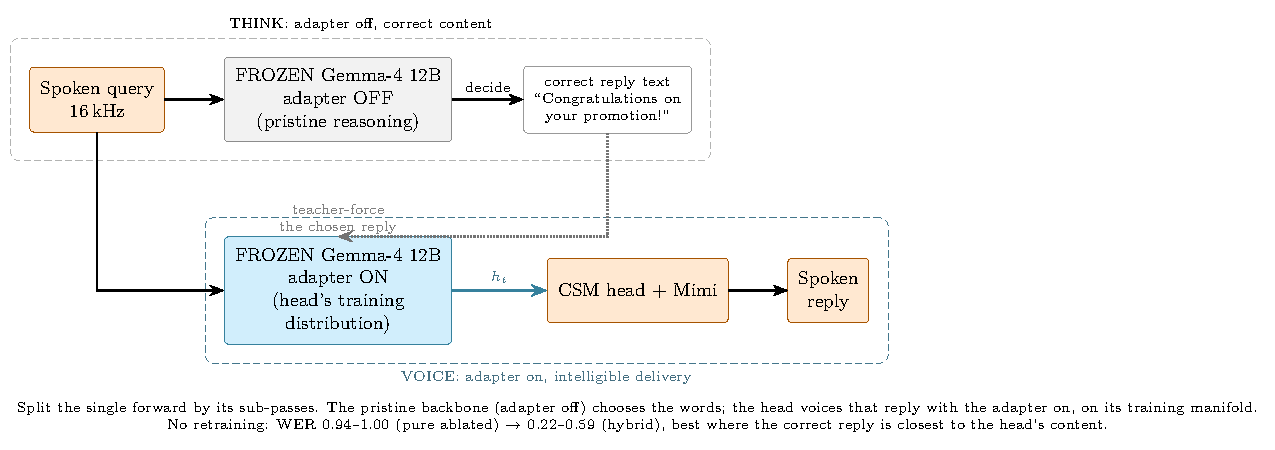
\includegraphics[width=\linewidth]{figures/hybrid.pdf}
\caption{The hybrid inference path. Ablate only the \emph{content-selection} sub-pass
(adapter off, so the frozen backbone reasons correctly), then voice the chosen reply
through the \emph{delivery} sub-pass with the adapter on, on the head's training manifold.
No weights change; it recovers correct content with largely intelligible speech where the
reply resembles the head's training content.}
\label{fig:hybrid}
\end{figure}

\paragraph{The trade-off.} This sharpens cascade-vs-unified into a genuine tension.
The cascade keeps the backbone's reasoning \emph{untouched}, only the head is
trained, preserving broad competence (91.9\% recall) at the cost of a text
bottleneck that discards prosody. The unified model removes that bottleneck (one
latent-conditioned forward, prosody-capable) but the adapter needed to wire the head
onto the latent perturbs the very reasoning we want to voice. The remedy is to touch
the ``thinker'' as little as possible: more and broader data, lighter or no LoRA, or
the in-trunk modality layers and limited unfreeze of
MOSS-Speech~\citep{zhao2025mossspeech}. The core claim, \emph{the model's own latent
reasoning, spoken aloud, from a single frozen encoder-free backbone}, is
demonstrated; making it robust out-of-distribution is a data-and-adaptation problem,
not an architectural one.

Realizing the \emph{single} end-to-end model hinged on getting delivery right.
A first attempt, wrapping the hand-spliced audio embeddings in the chat-template
framing tokens and training the joint objective end-to-end, does \emph{not}
suffice: although the teacher-forced text loss falls (to 2.3 held-out), the
free-running model \emph{bypasses the audio entirely}. Greedy decoding emits an
identical reply across all queries, and an ablation that zeros the audio leaves
that reply unchanged, so the response is independent of the input (the
teacher-forced trap of \S\ref{sec:findings} recurring at the system level). This
confirms that true native delivery requires the backbone's own multimodal forward
(audio soft-tokens placed by its \texttt{masked\_scatter}), not framing wrapped
around a manual splice. The working unified model of \S\ref{sec:unified} builds on
exactly this: it delivers audio through the native forward and conditions a
warm-started head on the resulting hidden states, which, unlike the splice,
suffices to produce intelligible, grounded, single-pass speech.

\subsection{Prosody conditioning: a weak loudness echo only}
\label{sec:prosody}
RQ2 in its original form asks whether the spoken reply tracks \emph{how} the query
was said. We test this directly with a minimal-pair probe on the splice path (the
path that carries prosody): for 12 held-out queries we hold the reply text fixed,
manipulate \emph{only} the input prosody into an ``aroused'' variant (higher pitch,
faster, louder) and a ``subdued'' one (the inverse) via DSP, generate $K{=}3$
samples per variant, and measure whether the output's F0, pitch range, intensity,
and duration shift in the input's direction, scored per-clip against the
temperature-0.7 sampling noise. The result is largely \emph{null}: output
\emph{intensity} weakly but consistently tracks input intensity (10/12 clips in the
expected direction, $p\approx0.02$; mean $\Delta{+}0.96$\,dB), while \emph{F0, pitch
range, and duration do not track at all} (mean deltas below the sampling-noise
floor, directional counts at chance). So although the splice delivers prosody into
the backbone, the text-conditioned speech head largely does not propagate it to
output prosody, only a faint loudness echo survives. Realising prosody
conditioning would require explicit prosodic supervision or the unified
native-delivery model (which has the query audio in-context during generation),
not the text-conditioned head as trained.

\subsection{Training stability: attention-sink NaN and optimizer poisoning}
\label{sec:stability}
Two instabilities cost real debugging time and generalize beyond this system.
\emph{(i) Attention-sink NaN.} The joint/grounded layouts place a raw audio
embedding at sequence position~0. Transformer decoders calibrate position~0 as an
attention sink (a massive-activation token, normally BOS); a raw audio embedding
there makes the backbone's RMSNorm \texttt{rsqrt} backward singular, producing a
\emph{NaN gradient from a finite loss}. Global gradient-norm clipping then
multiplies that single NaN into every parameter at the first optimizer step,
which looks like sudden whole-model corruption. \texttt{torch.autograd.set\_detect\_anomaly}
localizes it to RMSNorm; the fix is to prepend a BOS token so position~0 is
calibrated, plus a finiteness guard that skips any step with a non-finite
gradient norm. The transferable lesson: a finite loss does not imply finite
gradients, and clipping operates after the NaN already exists.
\emph{(ii) Optimizer poisoning on resume.} \texttt{PagedAdamW8bit} quantizes the
optimizer's second moment; a quantized near-zero variance makes the Adam update
$m/(\sqrt{v}{+}\epsilon)$ explode \emph{inside} the optimizer, downstream of
gradient clipping, so clipping cannot prevent it (a resumed run diverged to depth
loss ${>}200$). Resuming with a fresh full-precision optimizer (which fits on the
48\,GB rental, though not on 16\,GB) removes it.

\subsection{Key finding: $c_0$ is not intelligibility}
\label{sec:findings}
An early 12B Phase-A run on a small conversational corpus (OpenS2S) drove
teacher-forced $c_0$ to 1.3, which resembled our intelligibility breakthrough but
was memorization. Table~\ref{tab:c0wer} shows the dissociation: held-out $c_0$ is
far worse than trained $c_0$, and the decoded audio is unintelligible (141\% WER,
12\% recall) even where $c_0$ looks healthy.

\begin{table}[tbp]\centering
\caption{Teacher-forced $c_0$ versus free-running WER, OpenS2S Phase-A 12B.
Low $c_0$ coexists with garbled generation; only WER exposes it.}
\label{tab:c0wer}
\begin{tabular}{lccc}\toprule
 Model (training pairs) & $c_0$ trained & $c_0$ unseen & decoded WER \\ \midrule
 ckpt\_6000 \,(636)   & 2.31 & 8.18 &, \\
 ckpt\_14000 (2097)   & 1.56 & 2.09 & 141\% \\ \bottomrule
\end{tabular}
\end{table}

This dissociation mirrors \citet{penov2026loraBridges}: there, aggregate
language-modeling loss (bits-per-byte) cannot detect sensor conditioning, a
capacity-matched constant-feature control reproduces the entire metric gain, and
only task-aligned probes expose it. We observe the analogous gap between
teacher-forced $c_0$ (low even when the model cannot speak) and free-running WER,
which we therefore adopt as the gate. The same lesson recurs across the E2B
series: aggregate depth cross-entropy repeatedly failed to predict perceptual
quality, so word recall and blind listening, not loss curves, measure speech.

\subsection{Codec entropy floor}
\label{sec:codecfloor}
The acoustic (``depth'') loss plateaus at ${\sim}6.7$ and does not fall further.
Scaling the depth transformer from 150M to ${\sim}425$M parameters did not lower
the plateau, so it is not a capacity limit; it tracks Mimi's intrinsic
per-codebook entropy (${\sim}6.3$--$6.6$). M5 confirmed this independently: a
$30\times$ increase in the depth-loss weight ($0.01\to0.3$) produced \emph{zero}
reduction in held-out acoustic loss (validation depth flat at 6.55--6.60 across
2--10k steps), no intelligibility gain, and introduced stutter (repeated valid
codec frames, invisible to per-frame cross-entropy). Cross-entropy over discrete
RVQ codes therefore caps naturalness; closing it requires a flow-matching or
diffusion acoustic head over continuous features, not a loss-weight knob.

\section{Discussion \& Limitations}
\label{sec:discussion}
Three limitations stand out. First, the speech head is trained from scratch at
$d{=}3840$, so Phase A needs a large clean corpus; our OpenS2S misstep shows that
too little data produces a memorizing model that looks good on $c_0$ but cannot
speak. Second, naturalness is bounded by the codec floor (\S\ref{sec:codecfloor}),
not by model capacity or loss weighting; a continuous, flow-matching acoustic head
is the indicated next step. Third, single-16\,GB-GPU training is memory-bound: even
a rented A100 gave only ${\sim}1.5\times$ throughput, so scaling requires
configuration changes (sequence/precision/loader), not just a bigger card.
Fourth, while the unified single model is demonstrated (\S\ref{sec:unified}), one
native-delivery forward, intelligible and grounded full-length speech, its
out-of-distribution competence is eroded by adapter training: on prompts outside the
OpenS2S distribution it returns training templates, even though a three-way ablation
shows the frozen backbone's reasoning is intact (native Gemma and the adapter-disabled
model both answer correctly; only the trained LoRA masks it). The decisive delivery
insight still holds, a hand-built feature-splice carries prosody but not lexical
content, while the backbone's own multimodal pathway carries both, and the remaining
problem is preserving the backbone's latent reasoning while wiring the head onto it.
Concurrent text-free systems chart the route: Qwen2.5-Omni~\citep{xu2025qwen25omni}
conditions its speech generator on hidden representations from a genuine native
forward, and MOSS-Speech~\citep{zhao2025mossspeech} carves speech-prediction layers
into the trunk, frozen first, then partially unfrozen, on far more data, rather than
appending an external head behind a heavy adapter. Both point the same way as our
ablation: touch the ``thinker'' less (lighter or no LoRA, broader data, or in-trunk
modality layers), so the frozen backbone's reasoning survives into the spoken reply.

\section{Conclusion}
\label{sec:conclusion}
We show that lightweight adapters can teach a fully frozen, quantized LLM to speak
intelligibly (13\% WER), and that the same frozen, encoder-free backbone can hold a
spoken conversation through a two-stage cascade (native-pathway understanding into
the backbone, then a CSM-style speech head) with no backbone training. Along the way
we document five transferable findings. First, naive 4-bit quantization silently
destroys a multimodal backbone's audio comprehension while sparing prosody. Second,
\emph{how} audio is delivered (native pathway vs.\ hand-built feature-splice), not
quantization or capacity, decides whether lexical content survives. Third, a
convenient teacher-forced loss is not a proxy for the capability of interest, for
both speech and comprehension (WER on decoded audio is the gate). Fourth, a discrete
neural codec imposes an entropy floor that cross-entropy cannot cross. Fifth, when
the cascade is collapsed into a single native-delivery model, the frozen backbone's
reasoning stays intact but heavy adapter training masks it out-of-distribution: a
three-way ablation restores correct replies by disabling the adapter, so robustness
is a data-and-adaptation problem, not an architectural one. That single end-to-end
model, with the speech head conditioned on the backbone's own latent reply, speaks
intelligible, grounded, full-length replies in one forward pass, realizing the core
thesis of the model's own latent reasoning spoken aloud.

\section*{Reproducibility}
Code: \url{https://github.com/giannisanni/encoder-free-speech}. Checkpoints and data shards
are mirrored to HuggingFace (\texttt{giannisan/gemma-csm-ckpts},
\texttt{giannisan/gemma-csm-shards}). The appendix records the exact environment
and commands.

\bibliographystyle{plainnat}
\bibliography{references}

\appendix
\section{Reproducibility build-log}
\label{app:repro}
\paragraph{Backbone.} \texttt{google/gemma-4-12B-it}, \texttt{model\_type
gemma4\_unified}; \texttt{AutoModelForCausalLM} returns
\texttt{Gemma4UnifiedForConditionalGeneration}, whose \texttt{.model} is
\texttt{Gemma4UnifiedModel} (owns \texttt{get\_audio\_features}, \texttt{embed\_audio},
\texttt{language\_model}). Text config: hidden 3840, 48 layers, GQA 8 KV, no
per-layer-embedding tables, no KV-sharing. Audio config: hidden 640,
\texttt{audio\_embed\_dim} 640, \texttt{audio\_token\_id} 258881, up to 30\,s of
audio per input.

\paragraph{Environment.} A dedicated venv (\texttt{audioin-venv}): torch
2.11.0+cu128, torchvision, transformers built from source (5.13.0.dev0, which
ships \texttt{Gemma4UnifiedProcessor} / \texttt{Gemma4Unified\allowbreak Audio\allowbreak Feature\allowbreak Extractor}),
bitsandbytes, peft, pillow, soundfile, accelerate, datasets. The m-series used a
separate venv with transformers 5.10.2.

\paragraph{Data pipeline.} LJSpeech and LibriTTS are resampled to 24\,kHz mono and
Mimi-encoded (all 32 codebooks) into \texttt{\{id, text, codes\}} shards
(${\sim}18$ clips/s on the consumer card). OpenS2S English (49{,}368 pairs;
response audio ${\sim}71$\,GB across \texttt{en\_response\_wav.tar.gz.0--6}) is too
large to download; we stream first-encountered wavs from each tar (the tars are
not index-ordered) and intersect query/response/manifest indices, then re-encode
with Mimi. A chained multi-piece reader streams \texttt{.0}--\texttt{.6} as one
continuous gzip; a fresh \texttt{HfFileSystem} is required for the query pass
(closing the response handles tears down the shared HTTP client).

\paragraph{Training stability.} Checkpoints are written atomically
(\texttt{.tmp} then \texttt{os.replace}); a non-atomic save interrupted by a process
kill truncated a checkpoint and broke resume. \texttt{--resume} restores model,
step, and optimizer. A supervisor auto-resumes on death and frees VRAM (headless
target; stop GPU-resident side services) before each launch. Free-running decode
is gated with a silence-retry, and the run-log is appended (not truncated) across
restarts so the TensorBoard tail-follower stays continuous.

\end{document}
